\section{Other Features}
\subsection{Collision detectors}
\red{JS}
\subsection{Integration methods}
\red{Karen}
\subsection{Lazy evaluation and automatic update}
\label{sec:lazy}
Most kinematic libraries have a strict workflow that must be followed in order to produce correct results in a timely manner. Typically this workflow requires that all joint positions must be set, and then all transforms must be computed before the transformation of a specific frame may be queried. This is a wasteful and inefficient approach for many applications.

For example, a dexterous robot manipulator may have seven links from the base to the end effector, but then it may have three fingers which each have three links. While iteratively performing inverse kinematics, it will be necessary to repeatedly compute the seven matrix transformations that go from the base to the end effector, but the transforms of the nine finger links are unnecessary. A naive approach to updating kinematics will compute all 16 transforms, even though only 7 are necessary. This means that over 56\% of the computational effort of the forward kinematics is wasted. When iteratively solving an inverse kinematics problem, the bulk of time is spent computing forward kinematics. This means that intelligently updating the forward kinematics could yield a nearly 50\% reduction in computation time for this example.

Strict workflow requirements can also lead to bugs in code. If a human programmer is not familiar with the correct workflow, does not fully understand the \todo[MXG]{FINISH THIS}

\begin{figure}
  \centering
  \subfigure[][\label{fig:lazy_1}Everything is cached]{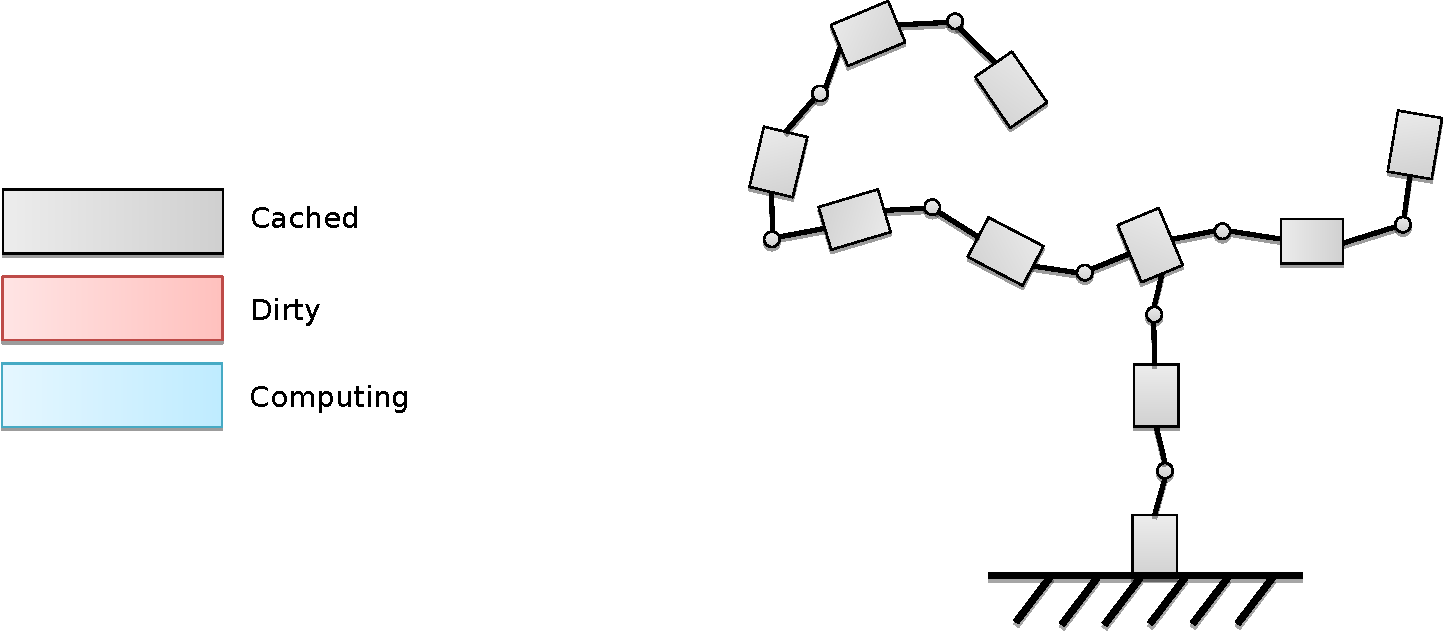
\includegraphics[width=0.98\textwidth]{fig/lazy_1.pdf}}
  
  \subfigure[][\label{fig:lazy_2}Some joint values have changed]{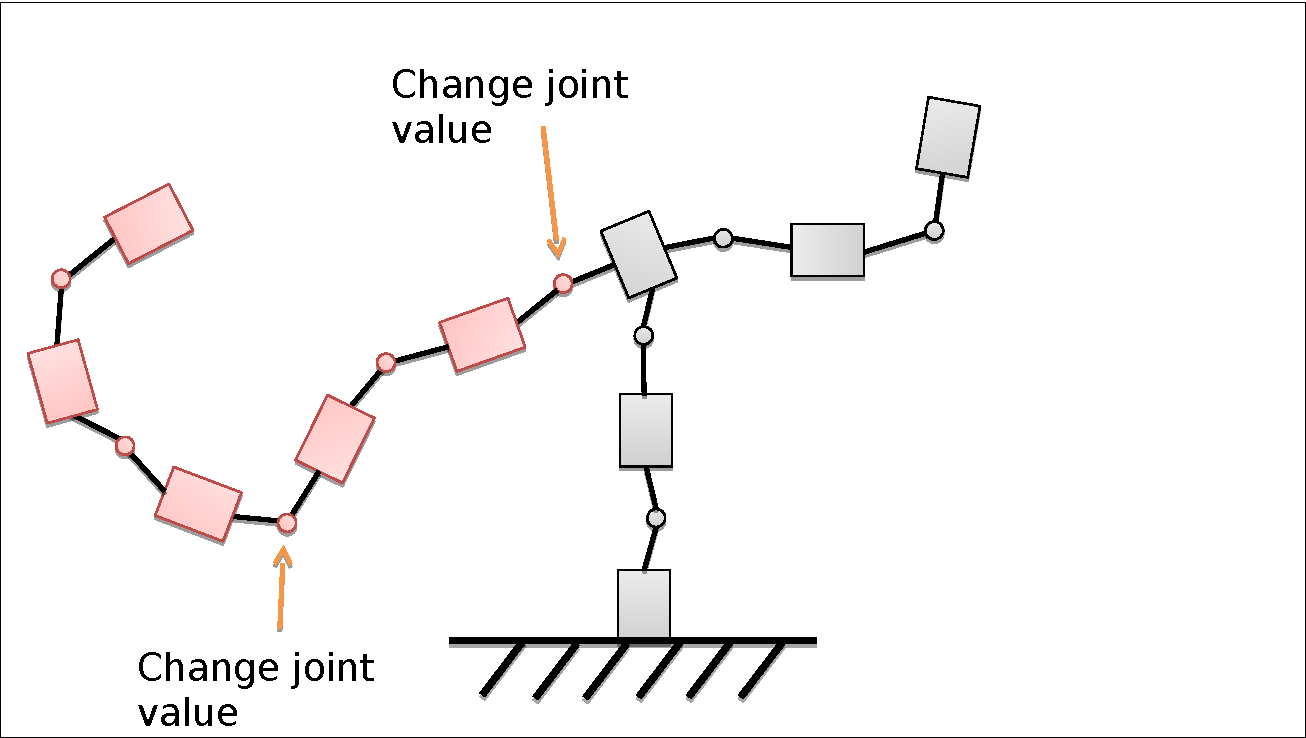
\includegraphics[width=0.44\textwidth]{fig/lazy_2.pdf}}
  \subfigure[][\label{fig:lazy_3}A dirty transform is queried]{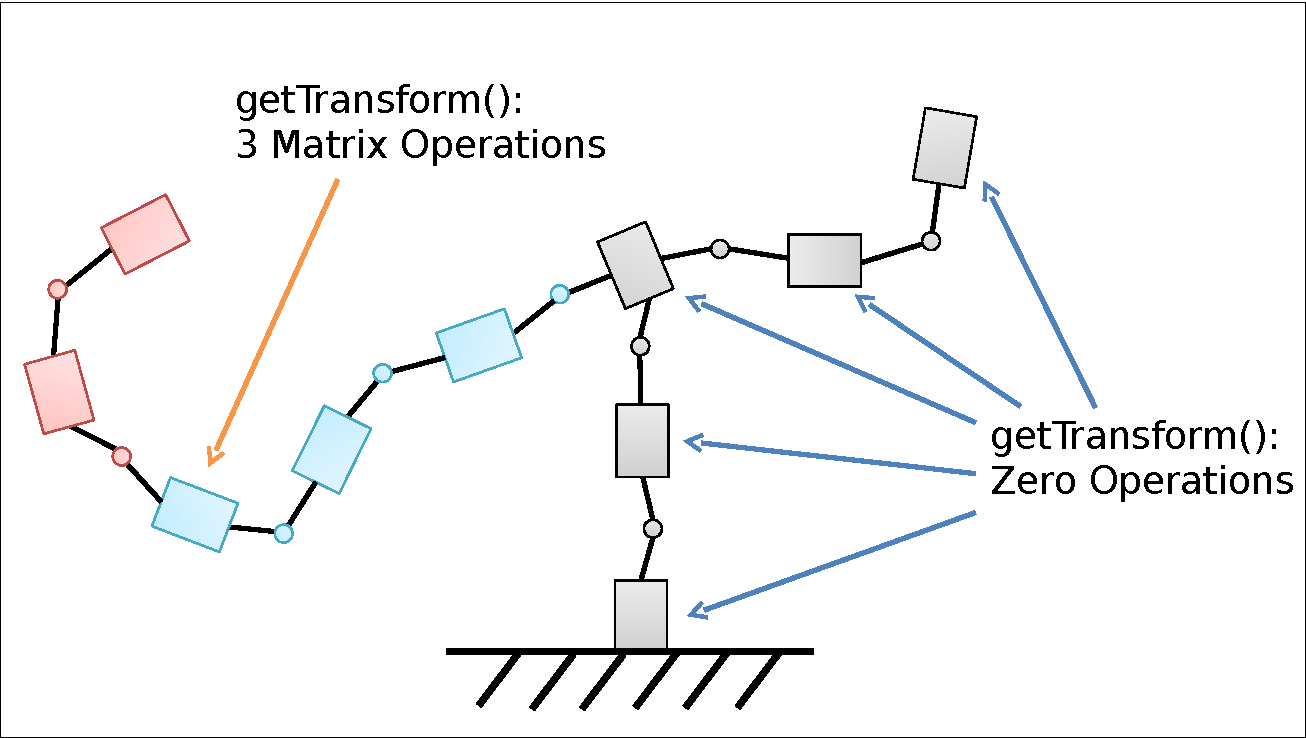
\includegraphics[width=0.44\textwidth]{fig/lazy_3.pdf}}
  
  \subfigure[][\label{fig:lazy_4}Cached transforms can be used freely]{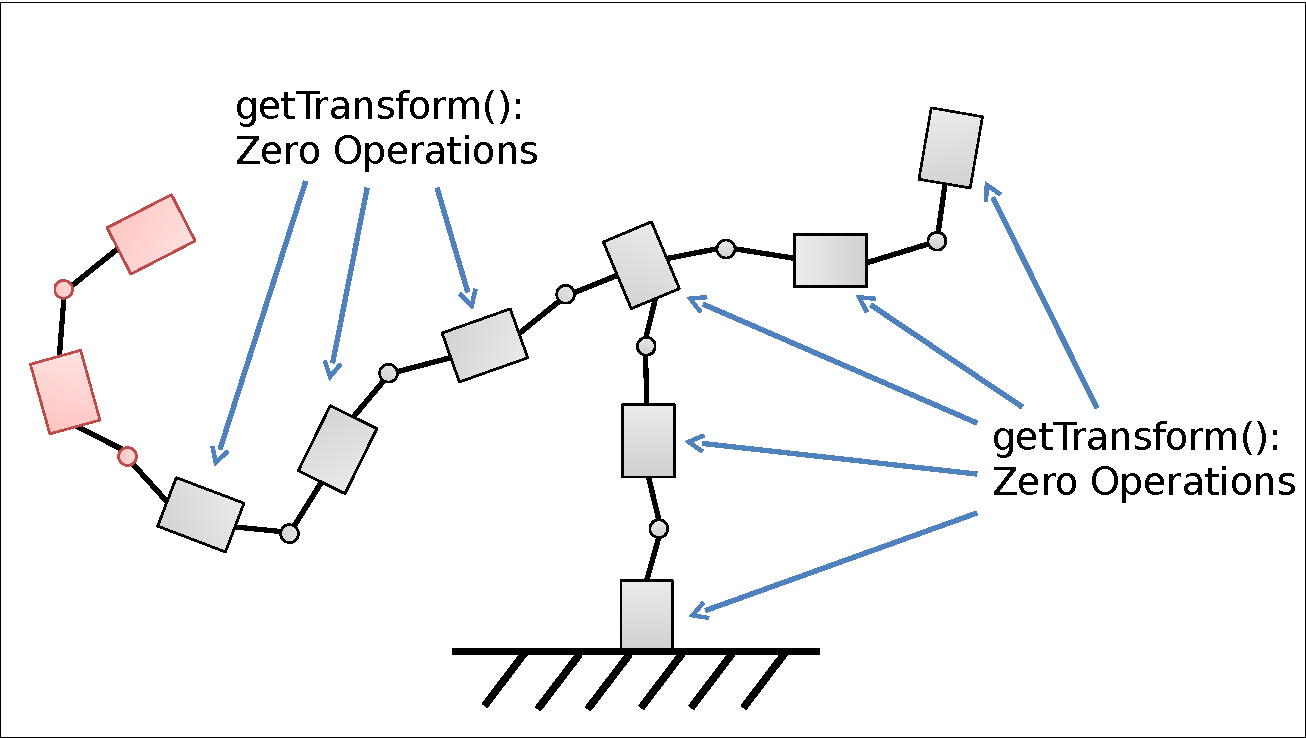
\includegraphics[width=0.44\textwidth]{fig/lazy_4.pdf}}
  \subfigure[][\label{fig:lazy_5}Another dirty transform is queried]{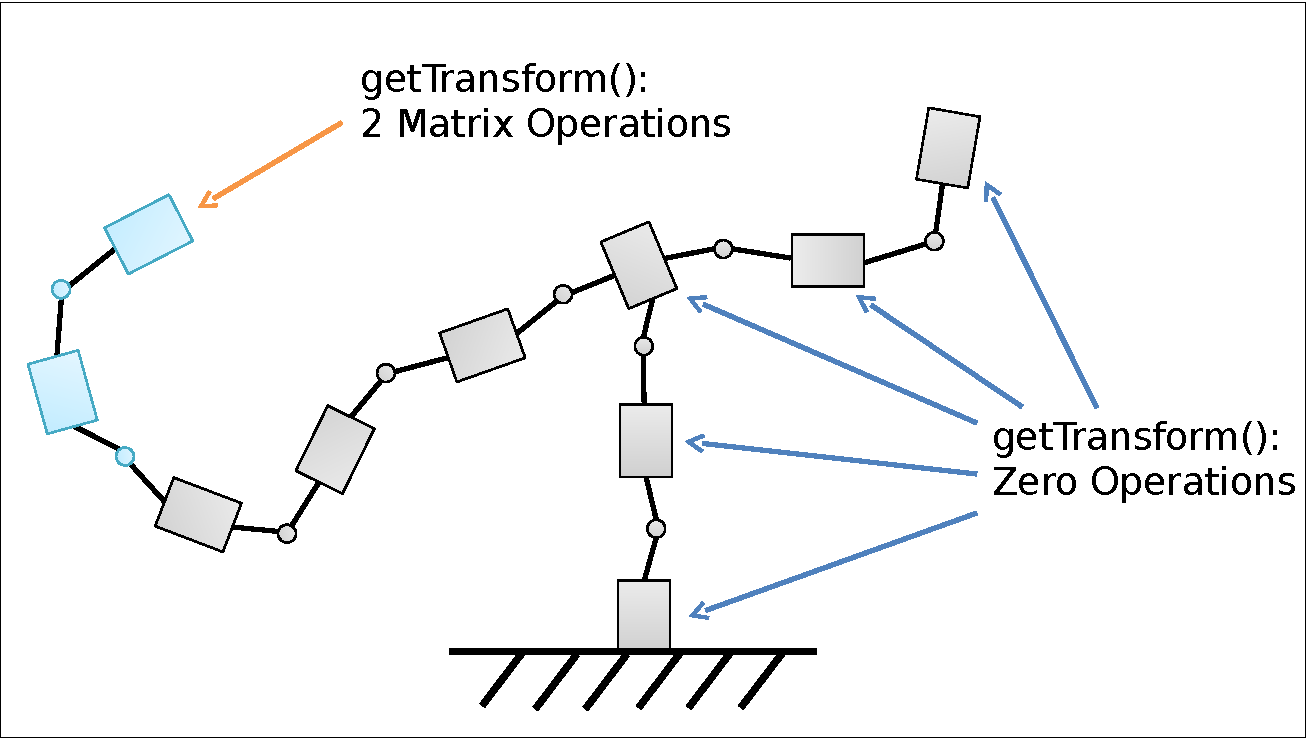
\includegraphics[width=0.44\textwidth]{fig/lazy_5.pdf}}
  \caption{Illustration of lazy evaluation for forward kinematics}
  \label{fig:red_ik}
\end{figure}

\subsection{Extensible data structures}
\subsubsection{Addons}
\label{sec:addons}
\subsubsection{Nodes}
\label{sec:nodes}
\red{Grey}
\subsection{History recorder}
\subsection{Optimization interface}
\label{sec:optimizer}
\red{Grey}
\subsection{Extensible GUI}
\red{JS}
